\documentclass[a4paper,12pt]{article}\usepackage[]{graphicx}\usepackage[]{xcolor}
% maxwidth is the original width if it is less than linewidth
% otherwise use linewidth (to make sure the graphics do not exceed the margin)
\makeatletter
\def\maxwidth{ %
  \ifdim\Gin@nat@width>\linewidth
    \linewidth
  \else
    \Gin@nat@width
  \fi
}
\makeatother

\definecolor{fgcolor}{rgb}{0.345, 0.345, 0.345}
\newcommand{\hlnum}[1]{\textcolor[rgb]{0.686,0.059,0.569}{#1}}%
\newcommand{\hlsng}[1]{\textcolor[rgb]{0.192,0.494,0.8}{#1}}%
\newcommand{\hlcom}[1]{\textcolor[rgb]{0.678,0.584,0.686}{\textit{#1}}}%
\newcommand{\hlopt}[1]{\textcolor[rgb]{0,0,0}{#1}}%
\newcommand{\hldef}[1]{\textcolor[rgb]{0.345,0.345,0.345}{#1}}%
\newcommand{\hlkwa}[1]{\textcolor[rgb]{0.161,0.373,0.58}{\textbf{#1}}}%
\newcommand{\hlkwb}[1]{\textcolor[rgb]{0.69,0.353,0.396}{#1}}%
\newcommand{\hlkwc}[1]{\textcolor[rgb]{0.333,0.667,0.333}{#1}}%
\newcommand{\hlkwd}[1]{\textcolor[rgb]{0.737,0.353,0.396}{\textbf{#1}}}%
\let\hlipl\hlkwb

\usepackage{framed}
\makeatletter
\newenvironment{kframe}{%
 \def\at@end@of@kframe{}%
 \ifinner\ifhmode%
  \def\at@end@of@kframe{\end{minipage}}%
  \begin{minipage}{\columnwidth}%
 \fi\fi%
 \def\FrameCommand##1{\hskip\@totalleftmargin \hskip-\fboxsep
 \colorbox{shadecolor}{##1}\hskip-\fboxsep
     % There is no \\@totalrightmargin, so:
     \hskip-\linewidth \hskip-\@totalleftmargin \hskip\columnwidth}%
 \MakeFramed {\advance\hsize-\width
   \@totalleftmargin\z@ \linewidth\hsize
   \@setminipage}}%
 {\par\unskip\endMakeFramed%
 \at@end@of@kframe}
\makeatother

\definecolor{shadecolor}{rgb}{.97, .97, .97}
\definecolor{messagecolor}{rgb}{0, 0, 0}
\definecolor{warningcolor}{rgb}{1, 0, 1}
\definecolor{errorcolor}{rgb}{1, 0, 0}
\newenvironment{knitrout}{}{} % an empty environment to be redefined in TeX

\usepackage{alltt} % This defines the style of your paper

\usepackage[top = 2.5cm, bottom = 2.5cm, left = 2.5cm, right = 2.5cm]{geometry} 

\usepackage[T1]{fontenc}
\usepackage[utf8]{inputenc}
% \usepackage{ctex}
\usepackage{amsthm, amsmath, amssymb, mathrsfs,mathtools}
\newtheorem{solution}{Solution}
\newtheorem{question}{Question}
\usepackage{color}

% The following two packages - multirow and booktabs - are needed to create nice looking tables.
\usepackage{multirow} % Multirow is for tables with multiple rows within one cell.
\usepackage{booktabs} % For even nicer tables.

% As we usually want to include some plots (.pdf files) we need a package for that.
\usepackage{graphicx} 
\usepackage{subfigure}


% The default setting of LaTeX is to indent new paragraphs. This is useful for articles. But not really nice for homework problem sets. The following command sets the indent to 0.
\usepackage{setspace}
\setlength{\parindent}{0in}


% Package to place figures where you want them.
\usepackage{float}

% The fancyhdr package let's us create nice headers.
\usepackage{fancyhdr}

\usepackage{fancyvrb}


%%%%%%%%%%%%%%%%%%%%%%%%%%%%%%%%%%%%%%%%%%%%%%%%
% 3. Header (and Footer)
%%%%%%%%%%%%%%%%%%%%%%%%%%%%%%%%%%%%%%%%%%%%%%%%

% To make our document nice we want a header and number the pages in the footer.

\pagestyle{fancy} % With this command we can customize the header style.

\fancyhf{} % This makes sure we do not have other information in our header or footer.

\lhead{\footnotesize EI071 Mathematics and Statistics For Economists}% \lhead puts text in the top left corner. \footnotesize sets our font to a smaller size.

%\rhead works just like \lhead (you can also use \chead)
\rhead{\footnotesize Jingle Fu, Chaitanya} %<---- Fill in your lastnames.

% Similar commands work for the footer (\lfoot, \cfoot and \rfoot).
% We want to put our page number in the center.
\cfoot{\footnotesize \thepage}
\IfFileExists{upquote.sty}{\usepackage{upquote}}{}
\begin{document}


\thispagestyle{empty} % This command disables the header on the first page. 

\begin{tabular}{p{15.5cm}} % This is a simple tabular environment to align your text nicely 
{\large \bf EI071 Mathematics and Statistics For Economists} \\
The Graduate Institute, Fall 2024, (Joy)Yang Jiao\\
\hline % \hline produces horizontal lines.
\\
\end{tabular} % Our tabular environment ends here.

\vspace*{0.3cm} % Now we want to add some vertical space in between the line and our title.

\begin{center} % Everything within the center environment is centered.
	{\Large \bf PS3 Solutions} % <---- Don't forget to put in the right number
	\vspace{2mm}
	
        % YOUR NAMES GO HERE
	{\bf Jingle Fu, Chaitanya Venkateswaran} % <---- Fill in your names here!
		
\end{center}  

\vspace{0.4cm}
\setstretch{1.5}

\section{R Code}
\begin{kframe}
\begin{alltt}
\hlcom{#1.1}
\hlkwd{data}\hldef{(mtcars)}

\hlcom{#1.2 }
\hlkwd{ncol}\hldef{(mtcars)}
\end{alltt}
\end{kframe}[1] 11
\begin{kframe}\begin{alltt}
\hlkwd{nrow}\hldef{(mtcars)}
\end{alltt}
\end{kframe}[1] 32
\begin{kframe}\begin{alltt}
\hlcom{#1.3}
\hlkwd{library}\hldef{(dplyr)}
\hldef{selected_data} \hlkwb{<-} \hlkwd{select}\hldef{(mtcars, mpg, cyl, hp)}
\hldef{mtcars} \hlopt \hlkwd{select}\hldef{(}\hlsng{'mpg'}\hldef{,} \hlsng{'cyl'}\hldef{,} \hlsng{'hp'}\hldef{)}
\end{alltt}
\end{kframe}                     mpg cyl  hp
Mazda RX4           21.0   6 110
Mazda RX4 Wag       21.0   6 110
Datsun 710          22.8   4  93
Hornet 4 Drive      21.4   6 110
Hornet Sportabout   18.7   8 175
Valiant             18.1   6 105
Duster 360          14.3   8 245
Merc 240D           24.4   4  62
Merc 230            22.8   4  95
Merc 280            19.2   6 123
Merc 280C           17.8   6 123
Merc 450SE          16.4   8 180
Merc 450SL          17.3   8 180
Merc 450SLC         15.2   8 180
Cadillac Fleetwood  10.4   8 205
Lincoln Continental 10.4   8 215
Chrysler Imperial   14.7   8 230
Fiat 128            32.4   4  66
Honda Civic         30.4   4  52
Toyota Corolla      33.9   4  65
Toyota Corona       21.5   4  97
Dodge Challenger    15.5   8 150
AMC Javelin         15.2   8 150
Camaro Z28          13.3   8 245
Pontiac Firebird    19.2   8 175
Fiat X1-9           27.3   4  66
Porsche 914-2       26.0   4  91
Lotus Europa        30.4   4 113
Ford Pantera L      15.8   8 264
Ferrari Dino        19.7   6 175
Maserati Bora       15.0   8 335
Volvo 142E          21.4   4 109
\begin{kframe}\begin{alltt}
\hlcom{#1.4}
\hldef{data1_4} \hlkwb{<-} \hlkwd{filter}\hldef{(mtcars, cyl} \hlopt{==} \hlnum{6}\hldef{, hp} \hlopt{>} \hlnum{100}\hldef{)}
\hldef{mtcars} \hlopt \hlkwd{filter}\hldef{(cyl} \hlopt{==} \hlnum{6}\hldef{, hp} \hlopt{>} \hlnum{100}\hldef{)}
\end{alltt}
\end{kframe}                mpg cyl  disp  hp drat    wt  qsec vs am gear carb
Mazda RX4      21.0   6 160.0 110 3.90 2.620 16.46  0  1    4    4
Mazda RX4 Wag  21.0   6 160.0 110 3.90 2.875 17.02  0  1    4    4
Hornet 4 Drive 21.4   6 258.0 110 3.08 3.215 19.44  1  0    3    1
Valiant        18.1   6 225.0 105 2.76 3.460 20.22  1  0    3    1
Merc 280       19.2   6 167.6 123 3.92 3.440 18.30  1  0    4    4
Merc 280C      17.8   6 167.6 123 3.92 3.440 18.90  1  0    4    4
Ferrari Dino   19.7   6 145.0 175 3.62 2.770 15.50  0  1    5    6
\begin{kframe}\begin{alltt}
\hlcom{#1.5}
\hldef{mtcars}\hlopt{$}\hldef{hp_per_cyl} \hlkwb{<-} \hldef{mtcars}\hlopt{$}\hldef{hp} \hlopt{/} \hldef{mtcars}\hlopt{$}\hldef{cyl}

\hlcom{#1.6}
\hldef{average_mpg} \hlkwb{<-} \hldef{mtcars} \hlopt
  \hlkwd{group_by}\hldef{(cyl)} \hlopt
  \hlkwd{summarize}\hldef{(}\hlkwc{avg_mpg} \hldef{=} \hlkwd{mean}\hldef{(mpg))}

\hlcom{#2.1}
\hlkwd{library}\hldef{(ggplot2)}
\hlkwd{ggplot}\hldef{(mtcars,} \hlkwd{aes}\hldef{(}\hlkwc{x} \hldef{= hp,} \hlkwc{y} \hldef{= mpg,} \hlkwc{color} \hldef{=} \hlkwd{as.factor}\hldef{(cyl)))} \hlopt{+}
  \hlkwd{geom_point}\hldef{()} \hlopt{+}
  \hlkwd{labs}\hldef{(}\hlkwc{color} \hldef{=} \hlsng{"Number of Cylinders"}\hldef{)}
\end{alltt}
\end{kframe}
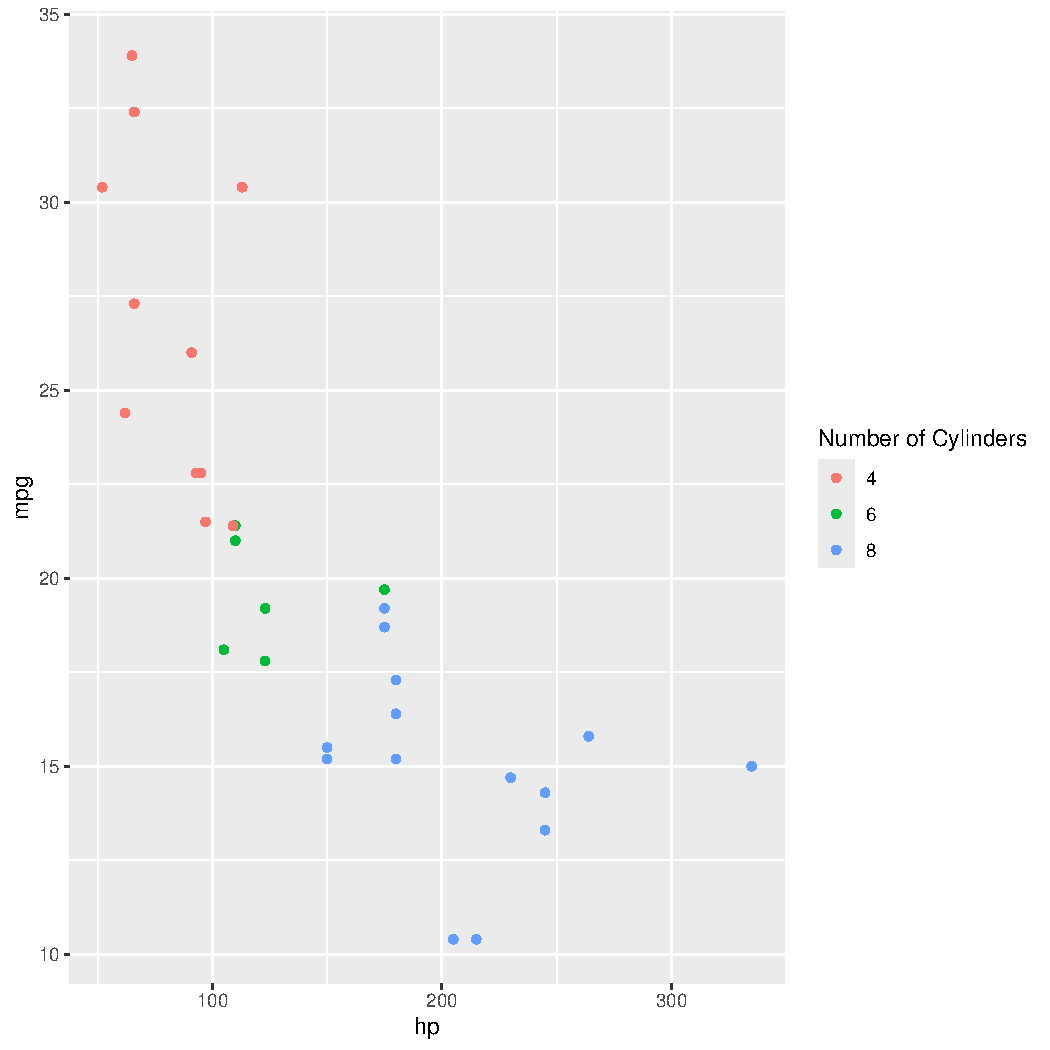
\includegraphics[width=\maxwidth]{figure/unnamed-chunk-1-1} 
\begin{kframe}\begin{alltt}
\hlcom{#2.2}
\hlkwd{ggplot}\hldef{(mtcars,} \hlkwd{aes}\hldef{(}\hlkwc{x} \hldef{=} \hlkwd{as.factor}\hldef{(cyl),} \hlkwc{y} \hldef{= mpg,} \hlkwc{fill} \hldef{=} \hlkwd{as.factor}\hldef{(cyl)))} \hlopt{+}
  \hlkwd{geom_boxplot}\hldef{()} \hlopt{+}
  \hlkwd{scale_fill_discrete}\hldef{(}\hlkwc{name} \hldef{=} \hlsng{"Number of Cylinders"}\hldef{)} \hlopt{+}
  \hlkwd{labs}\hldef{(}\hlkwc{x} \hldef{=} \hlsng{"Number of Cylinders"}\hldef{,} \hlkwc{y} \hldef{=} \hlsng{"Miles Per Gallon"}\hldef{)}
\end{alltt}
\end{kframe}
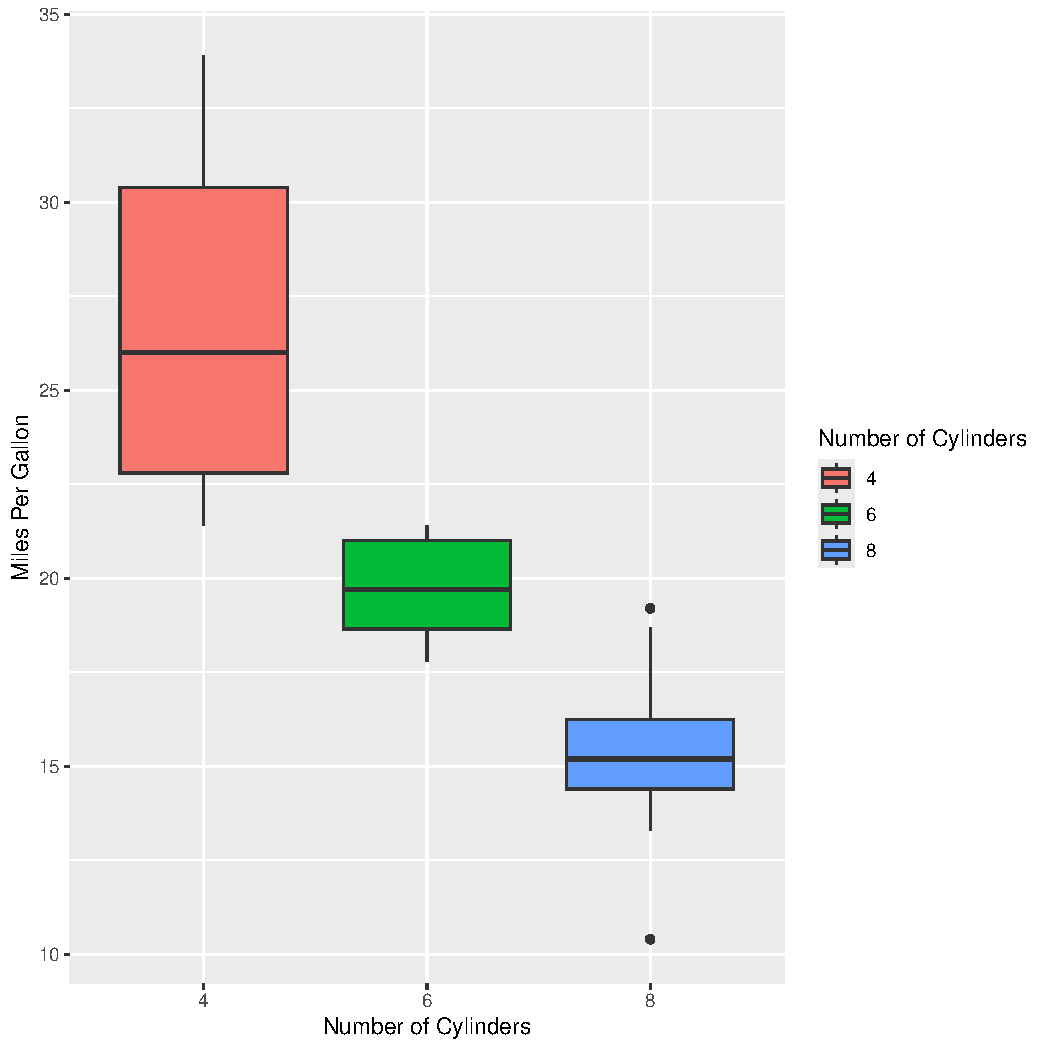
\includegraphics[width=\maxwidth]{figure/unnamed-chunk-1-2} 
\begin{kframe}\begin{alltt}
\hlcom{#2.3}
\hlkwd{ggplot}\hldef{(mtcars,} \hlkwd{aes}\hldef{(}\hlkwc{x} \hldef{= mpg))} \hlopt{+}
  \hlkwd{geom_histogram}\hldef{(}\hlkwc{binwidth} \hldef{=} \hlnum{2}\hldef{)} \hlopt{+}
  \hlkwd{xlab}\hldef{(}\hlsng{"Miles Per Gallon"}\hldef{)} \hlopt{+}
  \hlkwd{ylab}\hldef{(}\hlsng{"Frequency"}\hldef{)}
\end{alltt}
\end{kframe}
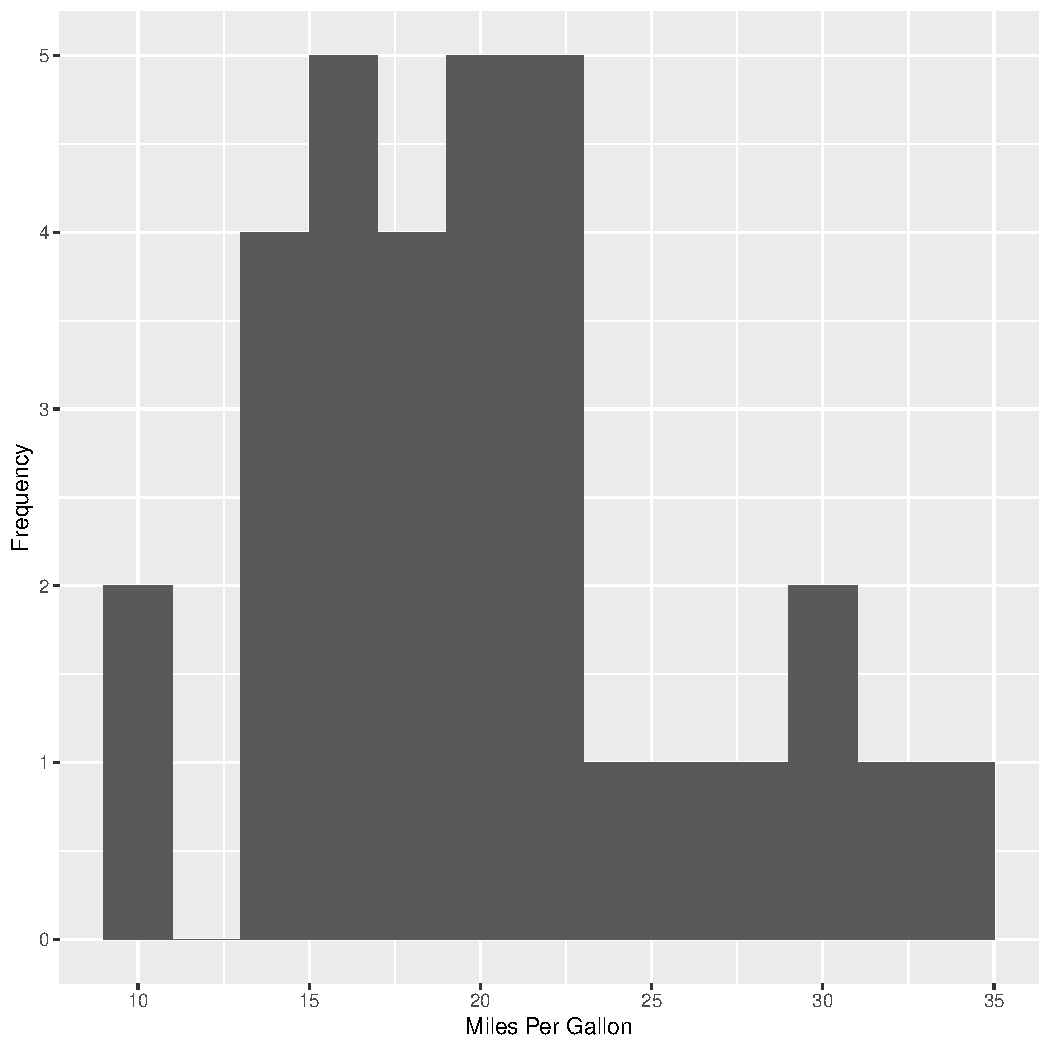
\includegraphics[width=\maxwidth]{figure/unnamed-chunk-1-3} 
\begin{kframe}\begin{alltt}
\hlcom{#3.1}
\hldef{mean_mpg} \hlkwb{<-} \hlkwd{mean}\hldef{(mtcars}\hlopt{$}\hldef{mpg)}
\hldef{mean_hp} \hlkwb{<-} \hlkwd{mean}\hldef{(mtcars}\hlopt{$}\hldef{hp)}

\hlcom{#3.2}
\hldef{var_mpg} \hlkwb{<-} \hlkwd{var}\hldef{(mtcars}\hlopt{$}\hldef{mpg)}
\hldef{var_hp} \hlkwb{<-} \hlkwd{var}\hldef{(mtcars}\hlopt{$}\hldef{hp)}

\hlcom{#3.3}
\hldef{cov_mpg_hp} \hlkwb{<-} \hlkwd{cov}\hldef{(mtcars}\hlopt{$}\hldef{mpg, mtcars}\hlopt{$}\hldef{hp)}

\hlcom{#3.4}
\hldef{cor_mpg_hp} \hlkwb{<-} \hlkwd{cor}\hldef{(mtcars}\hlopt{$}\hldef{mpg, mtcars}\hlopt{$}\hldef{hp)}

\hlcom{#4.1}
\hldef{car_names} \hlkwb{<-} \hlkwd{data.frame}\hldef{(}
  \hlkwc{car_model} \hldef{=} \hlkwd{rownames}\hldef{(mtcars),}
  \hlkwc{origin} \hldef{=} \hlkwd{c}\hldef{(}\hlkwd{rep}\hldef{(}\hlsng{'USA'}\hldef{,} \hlnum{10}\hldef{),} \hlkwd{rep}\hldef{(}\hlsng{'Europe'}\hldef{,} \hlnum{10}\hldef{),} \hlkwd{rep}\hldef{(}\hlsng{'Japan'}\hldef{,} \hlnum{12}\hldef{))}
\hldef{)}

\hldef{mtcars}\hlopt{$}\hldef{car_model} \hlkwb{<-} \hlkwd{rownames}\hldef{(mtcars)}
\hldef{merged_data} \hlkwb{<-} \hlkwd{merge}\hldef{(mtcars, car_names,} \hlkwc{by} \hldef{=} \hlsng{"car_model"}\hldef{)}

\hlcom{#4.2}
\hlkwd{library}\hldef{(tidyr)}
\hldef{long_format} \hlkwb{<-} \hlkwd{pivot_longer}\hldef{(mtcars,}
                            \hlkwc{cols} \hldef{=} \hlopt{-}\hldef{car_model,}
                            \hlkwc{names_to} \hldef{=} \hlsng{"variable"}\hldef{,}
                            \hlkwc{values_to} \hldef{=} \hlsng{"value"}\hldef{)}

\hlcom{#4.3}
\hldef{short_format} \hlkwb{<-} \hlkwd{pivot_wider}\hldef{(long_format,}
                            \hlkwc{names_from} \hldef{= variable,}
                            \hlkwc{values_from} \hldef{= value,}
                            \hlkwc{id_cols} \hldef{= car_model)}

\hlcom{#5.1}
\hlkwd{library}\hldef{(stargazer)}
\hldef{model} \hlkwb{<-} \hlkwd{lm}\hldef{(mpg} \hlopt{~} \hldef{hp} \hlopt{+} \hldef{wt,} \hlkwc{data} \hldef{= mtcars)}

\hlcom{#5.2}
\hlkwd{summary}\hldef{(model)}
\end{alltt}
\end{kframe}
Call:
lm(formula = mpg ~ hp + wt, data = mtcars)

Residuals:
   Min     1Q Median     3Q    Max 
-3.941 -1.600 -0.182  1.050  5.854 

Coefficients:
            Estimate Std. Error t value Pr(>|t|)    
(Intercept) 37.22727    1.59879  23.285  < 2e-16 ***
hp          -0.03177    0.00903  -3.519  0.00145 ** 
wt          -3.87783    0.63273  -6.129 1.12e-06 ***
---
Signif. codes:  0 '***' 0.001 '**' 0.01 '*' 0.05 '.' 0.1 ' ' 1

Residual standard error: 2.593 on 29 degrees of freedom
Multiple R-squared:  0.8268,	Adjusted R-squared:  0.8148 
F-statistic: 69.21 on 2 and 29 DF,  p-value: 9.109e-12

\begin{kframe}\begin{alltt}
\hlkwd{stargazer}\hldef{(model,} \hlkwc{type} \hldef{=} \hlsng{"latex"}\hldef{,}
          \hlkwc{out} \hldef{=} \hlsng{"PS3-5_2.tex"}\hldef{,}
          \hlkwc{title} \hldef{=} \hlsng{"Regression Results"}\hldef{,}
          \hlkwc{single.row} \hldef{=} \hlnum{TRUE}\hldef{,}
          \hlkwc{header} \hldef{=} \hlnum{FALSE}\hldef{,} \hlkwc{no.space} \hldef{=} \hlnum{TRUE}\hldef{)}
\end{alltt}
\end{kframe}
\begin{table}[!htbp] \centering 
  \caption{Regression Results} 
  \label{} 
\begin{tabular}{@{\extracolsep{5pt}}lc} 
\\[-1.8ex]\hline 
\hline \\[-1.8ex] 
 & \multicolumn{1}{c}{\textit{Dependent variable:}} \\ 
\cline{2-2} 
\\[-1.8ex] & mpg \\ 
\hline \\[-1.8ex] 
 hp & $-$0.032$^{***}$ (0.009) \\ 
  wt & $-$3.878$^{***}$ (0.633) \\ 
  Constant & 37.227$^{***}$ (1.599) \\ 
 \hline \\[-1.8ex] 
Observations & 32 \\ 
R$^{2}$ & 0.827 \\ 
Adjusted R$^{2}$ & 0.815 \\ 
Residual Std. Error & 2.593 (df = 29) \\ 
F Statistic & 69.211$^{***}$ (df = 2; 29) \\ 
\hline 
\hline \\[-1.8ex] 
\textit{Note:}  & \multicolumn{1}{r}{$^{*}$p$<$0.1; $^{**}$p$<$0.05; $^{***}$p$<$0.01} \\ 
\end{tabular} 
\end{table} 
\begin{kframe}\begin{alltt}
\hlcom{#5.3}
\hldef{predict_mpg} \hlkwb{<-} \hlkwd{predict}\hldef{(model,} \hlkwc{newdata} \hldef{=} \hlkwd{data.frame}\hldef{(}\hlkwc{hp} \hldef{=} \hlnum{150}\hldef{,} \hlkwc{wt} \hldef{=} \hlnum{3.0}\hldef{))}
\hlkwd{stargazer}\hldef{(predict_mpg,} \hlkwc{type} \hldef{=} \hlsng{"latex"}\hldef{)}
\end{alltt}
\end{kframe}
% Table created by stargazer v.5.2.3 by Marek Hlavac, Social Policy Institute. E-mail: marek.hlavac at gmail.com
% Date and time: 周二, 9月 17, 2024 - 22:48:56
\begin{table}[!htbp] \centering 
  \caption{} 
  \label{} 
\begin{tabular}{@{\extracolsep{5pt}} c} 
\\[-1.8ex]\hline 
\hline \\[-1.8ex] 
1 \\ 
\hline \\[-1.8ex] 
$20.828$ \\ 
\hline \\[-1.8ex] 
\end{tabular} 
\end{table} 
\begin{kframe}\begin{alltt}
\hlkwd{source}\hldef{(}\hlsng{"E:/IHEID国际经济学硕士/2024Fall/Mathematics and Statistics for Economists (EI071)/PS3.R"}\hldef{)}  \hlcom{# 确保路径是正确的}
\end{alltt}
\end{kframe}
\begin{table}[!htbp] \centering 
  \caption{Regression Results} 
  \label{} 
\begin{tabular}{@{\extracolsep{5pt}}lc} 
\\[-1.8ex]\hline 
\hline \\[-1.8ex] 
 & \multicolumn{1}{c}{\textit{Dependent variable:}} \\ 
\cline{2-2} 
\\[-1.8ex] & mpg \\ 
\hline \\[-1.8ex] 
 hp & $-$0.032$^{***}$ (0.009) \\ 
  wt & $-$3.878$^{***}$ (0.633) \\ 
  Constant & 37.227$^{***}$ (1.599) \\ 
 \hline \\[-1.8ex] 
Observations & 32 \\ 
R$^{2}$ & 0.827 \\ 
Adjusted R$^{2}$ & 0.815 \\ 
Residual Std. Error & 2.593 (df = 29) \\ 
F Statistic & 69.211$^{***}$ (df = 2; 29) \\ 
\hline 
\hline \\[-1.8ex] 
\textit{Note:}  & \multicolumn{1}{r}{$^{*}$p$<$0.1; $^{**}$p$<$0.05; $^{***}$p$<$0.01} \\ 
\end{tabular} 
\end{table} 



\end{document}
